\documentclass[border=2mm]{standalone}
\usepackage{pgfplots}
\usepackage[scaled]{helvet}
\usepackage[T1]{fontenc}
\renewcommand\familydefault{\sfdefault}
\usepackage[eulergreek]{sansmath}
\pgfplotsset{
tick label style = {font=\sansmath\sffamily}}

\pgfkeys{/pgf/number format/fixed}
\pgfplotsset{compat=newest}

\begin{document}

\pgfplotsset{
colormap={whitered}{color(0cm)=(white); color(1cm)=(orange!75!red)}}

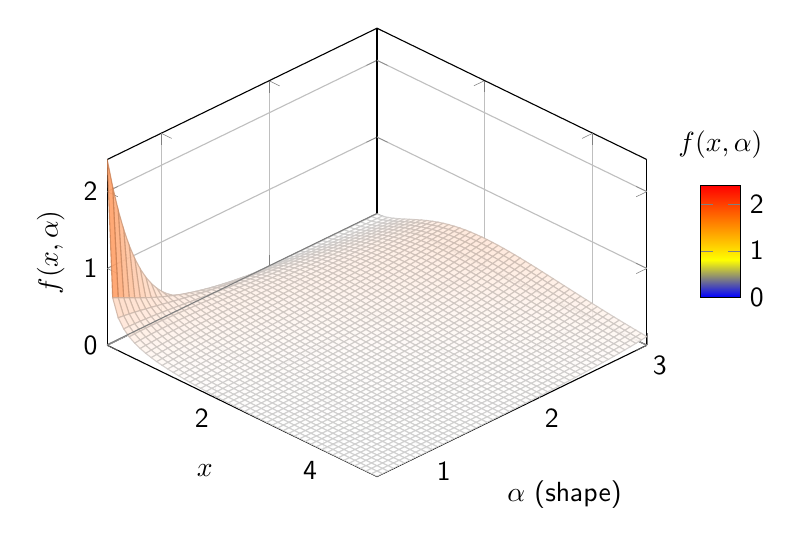
\begin{tikzpicture}[
    declare function={gamma_func(\z) = 2.506628274631*sqrt(1/\z) + 0.20888568*(1/\z)^(1.5) + 0.00870357*(1/\z)^(2.5) - (174.2106599*(1/\z)^(3.5))/25920 - (715.6423511*(1/\z)^(4.5))/1244160;}, % Stirling's approximation for gamma function
    declare function={gamma_pdf(\x,\alpha,\beta) = (\beta^\alpha)*(\x^(\alpha-1))*exp(-\beta*\x)/gamma_func(\alpha);}
]
\begin{axis}[
    view={45}{45},
    enlargelimits=false,
    grid=major,
    domain=0.01:5, % x values
    y domain=0.5:3, % shape parameter values
    samples=50,
    xlabel=$x$,
    ylabel=$\alpha$ (shape),
    zlabel={$f(x,\alpha)$},
    scaled z ticks=false,
    colorbar,
    colorbar style={
        at={(1.1,0.4)},
        anchor=south west,
        height=0.25*\pgfkeysvalueof{/pgfplots/parent axis height},
        scaled ticks=false,
        title={$f(x,\alpha)$}
    }
]
\addplot3 [surf, opacity=0.8, fill opacity=0.9, colormap={whitered}{color(0cm)=(white); color(1cm)=(orange!75!red)}, samples=50] {gamma_pdf(x,y,1)}; % using rate=1 for simplicity

\draw [black!50] (axis cs:0,0,0) -- (axis cs:5,0,0);
\draw [black!50] (axis cs:0,0,0) -- (axis cs:0,3,0);

\end{axis}
\end{tikzpicture}
\end{document}
